El problema de síntesis (construir automáticamente un controlador en base a una especificación) fue estudiado dentro de distintas áreas como: Discrete Event Control \textcolor{red}{[REFS]}, Reactive Synthesis \textcolor{red}{[REFS]} y Automated Planning \textcolor{red}{[REFS]}. El problema puede modelarse con un Sistema de Eventos Discretos (DES) con un subconjunto de sus estados marcados. Un factor clave de estos problemas es que el DES se presenta de forma modular tal que la composición paralela de múltiples componentes den lugar al DES de interés. Desarrollaremos en mayor detalle las definiciones del problema en el capítulo~\ref{chpt:background}.

La motivación para analizar dichos problemas surge de la necesidad de verificar software, hoy en día utilizado en prácticamente todo emprendimiento humano. Si bien puede irse ganando confianza sobre la correctitud de un algoritmo a través de una bateria de tests, éstos no proveen una garantía sino una seguridad cada vez mayor. 

Un método alternativo es el de la verificación de la implementación del algoritmo con un modelo formal que cumpla los objetivos y requerimientos deseados del programa. Con esta visión en mente, el área de `Controller Synthesis` va un paso más allá y busca la generación automática de un controlador que dado un modelo (en forma de DES) cumpla siempre en toda ejecución posible los requisitos del problema.

Podemos trazar una comparación con el método de "Machine Learning", en auge desde hace unos años. En este paradigma, el programa tiene como input una multitud de casos de ejemplo del comportamiento buscado, si ponemos como ejemplo ganar un juego de ajedrez, tomaría una biblioteca de partidas jugadas de las cuales aprender. Como resultado, presentaría un programa que sabe jugar al ajedrez "muy bien", es decir, es muy probable que dada una partida, la gane, pero no está garantizado. Pueden verse hoy en día muchas aplicaciones de este método con gran éxito, desde la dominación del juego del "go" hasta autos manejados por IA. Sin embargo, ya que no ofrece ninguna garantía, es un método poco apropiado para sistemas críticos.

Como contraste, la Síntesis de controladores toma como input las reglas del juego de ajedrez, por ejemplo, varios componentes (autómatas) separados, siendo cada uno los movimientos posibles para una pieza. Como resultado, daría un controlador, que en cada momento de la partida solo habilita algunas de las transiciones de los autómatas y garantiza que si se le hace caso ganará la partida. Es esencial notar que la técnica de este trabajo busca obtener una garantía muy fuerte, y el problema lo encuentra en la escalabilidad del problema, ya que hoy en día es imposible aplicarla a un juego del tamaño del ajedrez.

\section{Caso de estudio}\label{chpt:casoAviones}
A continuación se presenta un ejemplo para comprender el problema a resolver. Se trata de una versión simplificada del problema $Travel Agency$ utilizado para medir la performance del algoritmo.

Se desea armar un sevicio de venta online de paquetes vacacionales que reservará de forma automática una variedad de servicios (alquiler de auto, hotel, pasaje de avión, etc.) asegurando que no se perderá nada de dinero a menos que se reserve el paquete completo.

Para cada servicio que se desea sub-contratar presentamos una versión simplificada en la cual se consulta si ese servicio está disponible. En caso de estar disponible queda reservado hasta la compra definitiva del paquete completo y la cancelación de la reserva si otro servicio no estaba disponible no implica un gasto.

El problema puede escalar de forma muy rápida si se incrementa la cantidad de servicios a contratar o la cantidad de pasos para reservar cada servicio (como se verá en la sección~\ref{chpt:performance}).

Mostramos en la figura~\ref{fig:N1} un LTS (Labeled transition system) para cada uno de los componentes descriptos y el LTS compuesto para el caso en el que se sub-contrata un solo servicio.

Puede verse que para el caso de solo un sub-servicio que debe ser contratado el problema es manejable. Los modelos gráficos de la planta y el controlador, generados automáticamente por MTSA\footnote{Modal Transition System Analyser, \href{https://bitbucket.org/lnahabedian/mtsa/src/master/^}{https://bitbucket.org/lnahabedian/mtsa/src/master/}} se comprenden con un vistazo. Ya el caso con $N=2$ (fig~\ref{fig:N2}) si bien puede generarse una representación gráfica, requiere un trabajo considerable para comprender qué estado del problema representa cada estado del modelo. Simplemente aumentando a $N=5$ ya la planta compuesta cuenta con 1025 estados y 4085 transiciones. 

\begin{figure}[htb]
	\begin{center}
	\makebox[\linewidth][c]{%
	\begin{subfigure}[t]{.5\textwidth}
		\centering
		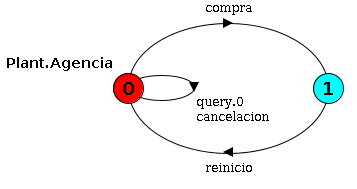
\includegraphics[width=\linewidth]{figures/ejemploServicios/agencia.png}  
		\caption{agencia}
		\label{fig:agencia}
	\end{subfigure}
	\begin{subfigure}[t]{.5\textwidth}
		\centering
		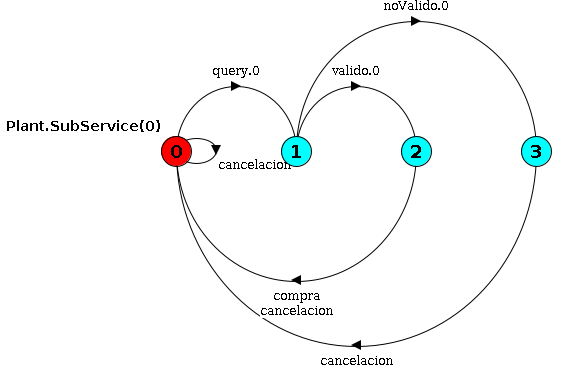
\includegraphics[width=\linewidth]{figures/ejemploServicios/subServicio.png}  
		\caption{un sub servicio}
		\label{fig:subserv}
	\end{subfigure}
	}
	\makebox[\linewidth][c]{%
	\begin{subfigure}[t]{.5\textwidth}
		\centering
		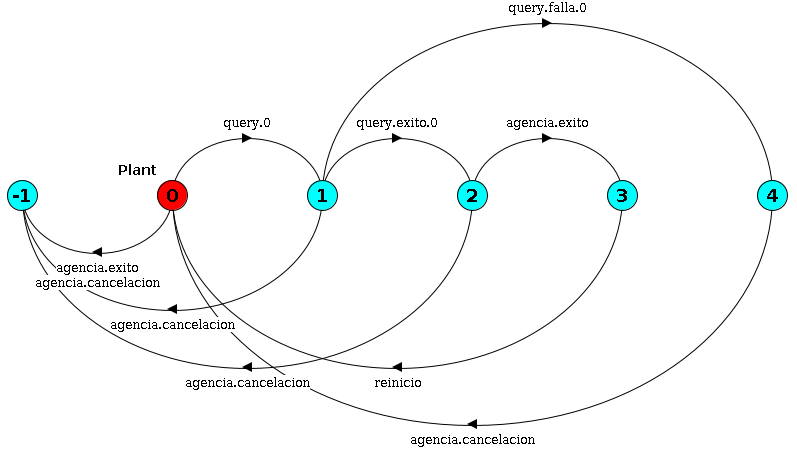
\includegraphics[width=\linewidth]{figures/ejemploServicios/N1Planta.png}  
		\caption{Planta compuesta}
		\label{fig:N1Planta}
	\end{subfigure}
	\begin{subfigure}[t]{.5\textwidth}
	\centering
	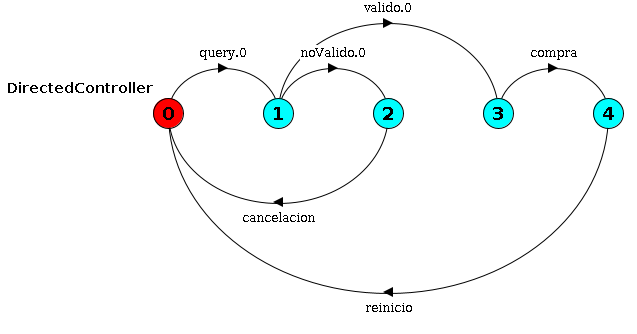
\includegraphics[width=\linewidth]{figures/ejemploServicios/N1Controlador.png}  
	\caption{Controlador resultante}
	\label{fig:controladorN1}
	\end{subfigure}
	}
	\caption{Caso con un solo sub-sevicio}
	\label{fig:N1}
	\end{center}
\end{figure}

\begin{figure}[htb]
	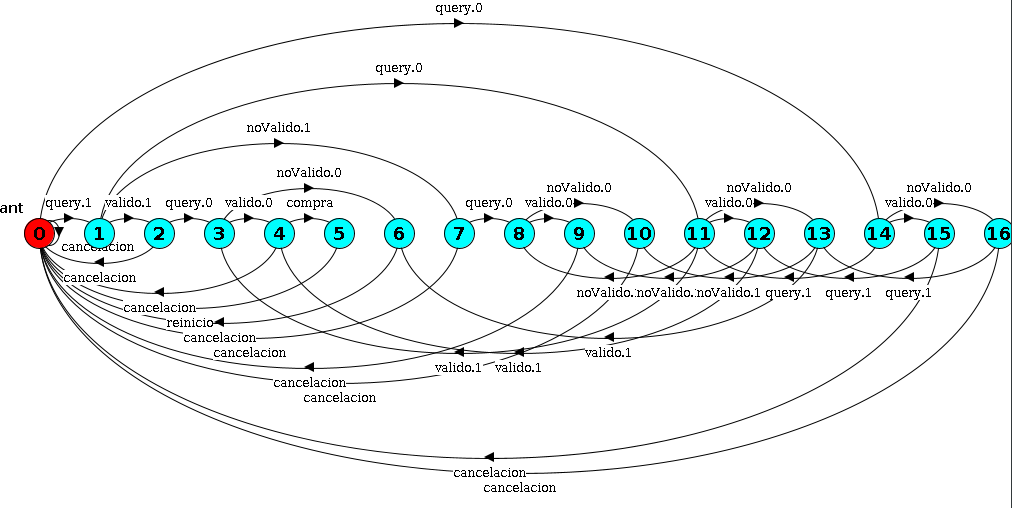
\includegraphics[width=\linewidth]{figures/ejemploServicios/N2Planta.png}  
	\caption{Planta compuesta con 2 sub-servicios}
	\label{fig:N2}
\end{figure}


Los algoritmos tradicionales necesitan construir el sistema compuesto entero antes de empezar, es por ésta explosión de estados y transiciones que resulta muy costoso (aveces imposible), por ende los algoritmos de punto fijo pueden manejar hasta cierto tamaño de problemas. En el caso de on-the-fly al ser una exploración dirigida construye sólo lo necesario, sacando conclusiones en función de la información obtenida; en el peor caso puede contruir todo (si es que esto es posible).

\section{Estructura de los capítulos}

En lo siguiente empezamos contando antecedentes, algoritmos tradicionales, la idea básica de exploración on-the-fly y lemas a seguir en orden de conseguir corrección y completitud; ésto puede encontrarse en el capítulo \ref{chpt:background}.

En el capítulo \ref{chpt:dcs} mostramos nuestra propuesta de algoritmo, demostramos corrección y completitud para el mismo y analizamos la complejidad computacional de su peor caso.

Luego exponemos detalles sobre la implementación en el capítulo \ref{chpt:implementation}, MTSA, heurísticas diseñadas para testeo y detalles sobre la batería de test, desarrollada utilizando TDD (Test Driven Development).

Como paso final en el capítulo \ref{chpt:performance} presentamos el benchmark utilizado y resultados de performance; tanto versus la versión anterior de DCS como versus otros algoritmos del estado del arte.










